\section{Adaptive  Exploration through Minimal Sample Complexity}\label{sec:lower_bound}
We seek to design a data collection strategy achieving minimal sample complexity.  Building on  BPI techniques \citep{garivier2016optimal,al2021navigating}, we first derive an instance-specific sample complexity lower bound for any $(\epsilon,\delta)$-PAC algorithm. 



This bound, which is posed as an optimization problem,  specifies the optimal exploration policy, enabling the derivation of an  efficient algorithm. The key step lies in bounding the expected log-likelihood ratio between the true model $M$ and a carefully constructed ``\emph{confusing}" model $M'$.


In the following section, we detail how these alternative models $M'$ are designed and leveraged to derive the sample complexity lower bound.


 

\subsection{Set of Alternative Models}
Confusing models are alternative models that are ``similar" to $M$, but differ in certain key properties. As we see later, the set of alternative models is crucial for establishing a lower bound on the sample complexity $\tau$.
 

To prove the lower bound, we frame the sample complexity problem as a goodness-of-fit test: does the observed data better align the true model $M$ or an alternative model $M'$?


The chosen model $M'$ is constructed to be \emph{confusing}—that is, it is close to $M$ (in the  KL sense), yet differs by at least $2\epsilon$ in the value of a policy $\pi$ under some reward $r$.


Formally, for a policy $\pi\in \Pi$, reward $r\in\rewardspace_\pi,$ the set of alternative models in $(\pi,r)$ is defined as
 \[{\rm Alt}_{\pi,r}^\epsilon(M) \coloneqq \{M_r': M\ll M_r', \; \|V_{M_r}^\pi - V_{M_r'}^\pi\|_\infty > 2\epsilon \},\] where for $M_r'=(\statespace, \actionspace,P_r',r,\gamma)$ the notation $M\ll M_r'$ means that $P(s,a)$ is absolutely continuous with respect to $ P_r'(s,a)$ for all $(s,a)$ (and $P$ is the transition function of $M$).  We also denote by ${\rm Alt}^\epsilon(M)=\cup_{\pi\in \Pi,r\in \rewardspace_\pi}{\rm Alt}_{\pi,r}^\epsilon(M)$ the entire set of alternative models over $\rewardspace$.
  
 From a sample complexity perspective, we can interpret this set as follows: a larger set of alternative models may lead to increased sample complexity since it becomes more likely that one of these models is close to $M$ as measured by their KL. Hence, we should expect the learning complexity to be dominated by the ``worst" among such models.


 
To gain more intuition, consider the case where the set ${\rm Alt}_{\pi,r}^\epsilon(M) = \emptyset$ is empty for some pair $(\pi,r)$. In this situation, any  model $P'$ sharing the same support as $P$ yields a value that is close to that of $P$. Thus, there is no  learning challenge for that reward. We'll see that characterizing when these sets are empty is crucial in our analysis. 



\paragraph{Value deviation.} To analyze these confusing sets, and their implications for sample complexity, we define the following instance-dependent quantity, that we refer to as the \emph{one-step value deviation}:
\begin{align*}\rho_r^\pi(s,s')&\coloneqq V_r^\pi(s') - \mathbb{E}_{\hat s \sim P(s,\pi(s))}[V_r^\pi(\hat s)] \quad\forall s,s'\in\statespace.
\end{align*}
This quantity measures how much the value at a state $s$ deviates from the expected value under $\pi$ as $s$. As we see later it is ``easier" to construct alternative models if $|\rho_r^\pi(s,s')|$ is large.

We also define these quantities in vector form
$
\rho_r^\pi(s) \coloneqq \begin{bmatrix}
    \rho_r^\pi(s,s_1) &\dots &\rho_r^\pi(s,s_S)
\end{bmatrix}^\top$,
so that $\|\rho_r^\pi(s)\|_\infty= \max_{s'} |\rho_r^\pi(s,s')|$ is the maximum
one-step deviation at $s$. 
The deviation $\rho_r^\pi$ is closely related to the \emph{span} of the value function $
    {\rm sp}(V_r^\pi) \coloneqq \max_{s'}V_r^\pi(s')-\min_{s'} V_r^\pi(s)$,
but, is in general smaller, as discussed  in \cref{app:value_deviation}.

Using this measure of value deviation  $\rho_r^\pi$, we are able to provide a necessary and sufficient conditions under which ${\rm Alt}_{\pi,r}^\epsilon(M)$ is empty (see proof in \cref{app:prop:suffnecc_cond_confusing_models}).
\begin{tcolorbox}
\begin{proposition}\label{prop:suffnecc_cond_confusing_models}
   Let $\pi\in \Pi,r \in \mathcal{R}_\pi$. The set ${\rm Alt}_{\pi,r}^\epsilon(M)$ is empty if and only if
   \[\frac{2\epsilon(1 - \gamma)}{\gamma } \geq \max_{s\in \statespace} \|\rho_r^\pi(s)\|_\infty.
   \]
\end{proposition}
\end{tcolorbox}
The proposition provides insights into the challenges of learning the value function:

\begin{itemize}
    \item  As $\epsilon$ increases, or $\gamma$ decreases, the condition in \cref{prop:suffnecc_cond_confusing_models} is  more likely to be satisfied, meaning that  the number of possible confusing models may increase. This fact could imply an increase in the sample complexity.
    
    \item The proof introduces the notion of \emph{confusing} states: a state $s$ is confusing if
    $
        \frac{\epsilon(1 - \gamma)}{\gamma \|\rho_r^\pi(s)\|_\infty} < 1
    $. A smaller value of $\|\rho_r^\pi(s)\|_\infty$ implies that state $s$ does not significantly influence the sample complexity. Additionally, \cref{lemma:bound_rho} (in the appendix) suggests that $\max_{s'} |\rho_r^\pi(s,s')|$ is unlikely to be attained at $s=s'$.
\item 
Since $|\rho_r^\pi(s,s')|\leq {\rm sp}(V_r^\pi)$ (see \cref{lemma:bound_rho} in the appendix),  similar values across states lead to lower sample complexity.

    
    \item Finally, if $\max_{s\in \statespace}\|\rho_{r}^\pi(s)\|_\infty = 0$, then ${\rm Alt}_{\pi,r}^\epsilon(M)$ is empty regardless of the values of $\epsilon$ and $\gamma$.
\end{itemize}

Regarding the last point, in the following proposition, proved in \cref{app:prop:rho_zero_ness_succ}, we provide a sufficient and necessary condition for $\max_s\|\rho_r^\pi(s)\|_\infty=0$.

\begin{tcolorbox}
\begin{proposition}\label{prop:rho_zero_ness_succ}
    The vectors $r$ for which $\max_{s} \|\rho_r^\pi(s)\|_\infty=0$ is precisely the subspace $\{\alpha {\bf 1} : \alpha \in [0,1]\}$, where ${\bf 1}$ is the vector of ones. 
    %Thus, $r$ must be a scalar multiple of ${\bf 1}$.
\end{proposition}
\end{tcolorbox}
While it may seem obvious that the unit vector reward cannot produce an alternative model, it is noteworthy  that no other reward satisfies $\max_{s} \|\rho_r^\pi(s)\|_\infty=0$ for any MDP.

We are now ready to discuss the sample complexity, and we refer the reader to \cref{app:prop:rho_zero_ness_succ} for further discussion on the set of alternative models, including a characterization of when $\rho_r^\pi(s,s)$ is identically zero across all states. 



 
\subsection{Sample Complexity Lower Bound} 
As a  consequence of \cref{prop:suffnecc_cond_confusing_models}, the analysis of the sample complexity must necessarily take into account the set of rewards. We let $\rewardspace_\pi^\epsilon =\{r\in \rewardspace_\pi: {\rm Alt}_{\pi,r}^\epsilon(M) \neq \emptyset\}$ be the set of rewards for which the corresponding set of confusing models is non-empty.

To derive the sample complexity lower bound, we also define the \emph{characteristic time} $ T_\epsilon(\omega;M)$ of a stationary state-action distribution $\omega$ under $M$:\begin{equation}\label{eq:T_epsilon_omega} T_\epsilon(\omega;M)^{-1}\coloneqq \inf_{\pi\in \Pi,r\in \rewardspace_\pi^\epsilon, M_r'\in {\rm Alt}_{\pi,r}^\epsilon(M)}\mathbb{E}_{\omega}[{\rm KL}_{P|P_r'}(s,a)], \end{equation}
where the inverse of $ T_\epsilon(\omega;M)$ can be thought of as \emph{information rate}, i.e., the amount of information gathered per time-step under $\omega$.
Then, one can show that asymptotically the sample complexity lower bound for any $(\epsilon,\delta)$-PAC algorithm scales according to  \begin{equation}\label{eq:T_star}
    T_\epsilon^\star(M) = \min_{\omega \in \Omega(M)} T_\epsilon(\omega;M)
\end{equation}
where   we    denote by $\omega_{\rm opt}$ the  solution to the optimization in Eq. (\ref{eq:T_star}), and $\Omega(M)$  is defined as the set of state-action distributions satisfying the forward equations:
$\Omega(M)\coloneqq \Big\{\omega\in \Delta(\statespace\times\actionspace):  \sum_{a} \omega(s,a) = \sum_{s',a'} P(s|s',a'),\omega(s',a')\;\forall s \Big\}.$
 We have the following asymptotic lower bound, and the proof of the theorem can be found in \cref{app:thm:sample_complexity_lb}.
 \begin{tcolorbox}
\begin{theorem}\label{thm:sample_complexity_lb}For any $(\epsilon,\delta)$-PAC algorithm we have \begin{equation}\label{eq:lower_bound}
    \liminf_{\delta \to 0}\frac{\mathbb{E}[\tau]}{\log(1/\delta)} \geq T_\epsilon^\star(M).
    \end{equation}
\end{theorem}
\end{tcolorbox}
Though the result may at first appear abstract, it provides  insights into the challenges of exploration. The optimal exploration strategy $\omega_{\rm opt}$, in terms of state-action visitations,  maximizes information gain per time-step  required to  distinguish between the true model $M$ and a confusing one.

This problem can be framed conceptually as a zero-sum game:  the explorer seeks to maximize $T_\epsilon(\omega; M)^{-1}$ over $\omega$, while an adversary selects a confusing model for some policy–reward pair to minimize this value. Consequently, the sample complexity is determined by the most difficult policy–reward pair to discriminate from the true model.

 
 However, it it may seem counterintuitive to use an exploration strategy that depends on the true model itself $M$, since it is unknown. In practice,  we use the empirical estimate of the MDP $M_t$ at timestep $t$ to derive an exploration strategy. We defer this discussion to \cref{sec:algorithms}. 

This result also reveals under which conditions a data collection policy \(\pi_\beta\) is optimal  up to a constant. Due to space constraints, we defer this discussion to \cref{app:optimality_behavior_policies}. Generally, we find that \(\pi_\beta\) must induce a stationary distribution \(d^{\pi_\beta}\) that  samples states with larger values of  \(\|\rho_r^\pi(s)\|_\infty\).



Last, but not least, the lower bound expression does not clearly reveal its scaling behavior or its connection to the value deviation \(\rho\). While we have briefly touched upon this relationship, these aspects are explored in greater depth in the next section, where a convexification of the problem provides further insights into these properties. 





\subsubsection{Convexity of the Lower Bound}
We find that it is hard to directly optimize $T_\epsilon(\omega;M)$, since the optimization  the set of alternative models may be non-convex.
Observe  that  the set ${\rm Alt}_{\pi,r}^\epsilon(M)$ can be seen as the union of two sets $\{M': \max_s V_{M_r}^\pi(s) - V_{M_r'}^\pi(s) \geq 2\epsilon\}$ and  $\{M': \max_s  V_{M_r'}^\pi(s) - V_{M_r}^\pi(s) \geq 2\epsilon\}$. The convexity of these sets depend on $(\pi, r, P)$ and, even if convex, may be disjoint. The following example illustrates this aspect.
\begin{figure}[b]
    \centering
      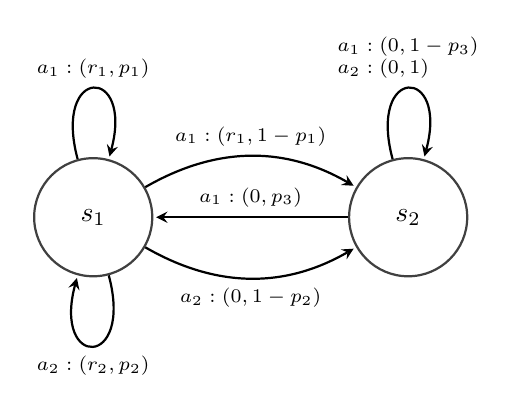
\begin{tikzpicture}[->,>=stealth,shorten >=1pt,auto,node distance=2cm,thick]
        \tikzstyle{state}=[circle,thick,draw=black!75,minimum size=15mm,inner sep=2mm]
        
        \node[state] (A) at (0,0) {$s_1$};
        \node[state] (B) at (4,0) {$s_2$};
        
        \path (A) edge [loop above] node[midway,above, font=\scriptsize] {$a_1:(r_1,p_1)$} 
        (A) edge [loop below] node[midway,below, font=\scriptsize] {$a_2:(r_2,p_2)$} 
        (A)  edge [bend left]  node[midway,above, font=\scriptsize] {$a_1:(r_1,1-p_1)$} (B)
        (B)  edge [out=180, in=360]  node[midway,above, font=\scriptsize] {$a_1:(0,p_3)$} (A)
         (A)  edge [bend right] node[midway,below, font=\scriptsize] {$a_2:(0,1-p_2)$} (B)
    (B) edge [loop above] node[midway,above, font=\scriptsize,align=left] {%
    $a_1:(0,1-p_3)$\\$a_2:(0,1)$} (B);
    \end{tikzpicture}
        \caption{In this MDP (v. \cref{example:non_convexity}),  in each edge it is indicated the action and the corresponding reward and transition probability.}
        \label{fig:example_non_convex_mdp}
\end{figure}
\begin{example}\label{example:non_convexity}
Consider the MDP in \cref{fig:example_non_convex_mdp} with the target policy \(\pi(s_1) = a_2\) and \(\pi(s_2) = a_1\). The value functions are given by
$\
V^\pi(s_2) = \theta V^\pi(s_1)$, where $\theta = \frac{\gamma p_3}{1 - \gamma(1 - p_3)}$, 
and
$
V^\pi(s_1) = \frac{p_2 r_2}{1 - \gamma(p_2 + (1 - p_2)\theta)}.
$
Using parameters \(\gamma = 0.9\), \(r_2 = \frac{1}{2}\), \(p_3 = 10^{-2}\), and \(p_2 = \frac{1}{2}\) in the true model \(M\), consider an alternative model \(M'\) with the same \((p_1, r_1, r_2, \gamma)\). Varying \(p_2\) in \(M'\) shows that \(p_2 = 0.56\) and \(p_2 = 0.41\) are both confusing for \(\epsilon = 0.03\), whereas their average is not. This phenomenon is illustrated in \cref{fig:non-convexity-example-plot}.
\end{example}

In the next sub-section we explain how to circumvent this issue by considering a convex relaxation of the optimization problem in Eq. \ref{eq:T_epsilon_omega}, denoted as the \emph{relaxed characteristic time}.


\subsection{Relaxed Characteristic Time}
\begin{figure}[t]
    \centering
    \includegraphics[width=.55\linewidth]{figures/example_non_convexity.pdf}
    \caption{Plot of $\|V_{M}^\pi-V_{M'}^\pi(p_2)\|_\infty$ for varying values of $p_2$ in $M'$ (the other parameters are the same in both MDPs). The parameters $p_{2a}=0.56$ and $p_{2b}=0.41$ are both confusing parameters for $\epsilon=0.03$ (above the red line), but their average $p_{2m}$ is not.}
    \label{fig:non-convexity-example-plot}
\end{figure}
We proceed with finding a convex relaxation of $T_\epsilon(\omega;M)$ that holds for all distributions $\omega\in \Delta(\statespace\times \actionspace)$.
Such relaxation not only upper bounds $T_\epsilon(\omega;M)$  in terms of $\rewardspace_\pi$ (instead of $\rewardspace_\pi^\epsilon$), but also allows   to better understand the scaling of $T_\epsilon^\star$. The proof can be found in \cref{app:thm:relaxed_characteristic_time}.
\begin{tcolorbox}
\begin{theorem}\label{thm:relaxed_characteristic_time}
    For all $\omega\in \Delta(\statespace\times \actionspace)$ we have $T_\epsilon(\omega;M)\leq U_\epsilon(\omega;M)$, where
    \begin{equation}
U_\epsilon(\omega;M)\coloneqq \sup_{\pi\in \Pi,r\in {\cal R}_\pi} \max_{s\in\statespace} \frac{\gamma^2 \|\rho_r^\pi(s)\|_\infty^2}{4\epsilon^2 (1-\gamma)^2 \omega(s,\pi(s))},
    \end{equation}
 is convex in $\omega$.
Let  $U_\epsilon^\star(M) = U_\epsilon(\omega^\star;M)$ be the optimal  rate, where $\omega^\star=\argmin_{\omega\in \Omega(M)}U_\epsilon(\omega;M)$ is the $U_\epsilon$-optimal visitation strategy.
\end{theorem}
\end{tcolorbox}
This theorem exhibits some of the characteristics we mentioned before: as expected, the complexity is characterized by  pairs $(s,s')$ for which the   deviation $|\rho_r^\pi(s,s')|$  is large, for some worst-case policy-reward pair. 
What this result suggests, is that sampling should be roughly proportional to the value deviation (a quantity that  is a variance-like measure, as explained also in \cite{russo2023model}). However, quantifying the gap $|U_\epsilon(\omega;M)-T_\epsilon(\omega;M)|$ remains challenging, and we leave this analysis to future work.

Solving this optimization problem is straightforward:  when each ${\cal R}_\pi$ is finite, it can be formulated within the framework of disciplined convex programming (DCP) \cite{grant2006disciplined}. Furthermore, the problem remains convex when the sets ${\cal R}_\pi$ are convex, and can still be solved using DCP. In particular, under the reward-free scenario ${\cal R}_\pi=[0,1]^S, \forall \pi \in \Pi$, the  optimization in $r$ admits a closed-form solution, as we discuss in the next subsection.


\subsubsection{Optimization over a Convex Set of Rewards}
For a convex reward set $\mathcal{R}_\pi$, the optimization  in 
\cref{thm:relaxed_characteristic_time} can be formulated as a convex problem in $r$. 
Additionally, we derive a closed-form solution for reward-free policy evaluation when $\rewardspace = [0,1]^S$. In this case the solution is defined by the matrix $\Gamma_{i,j}^\pi(s) = \left(K^\pi(s) G^\pi\right)_{i,j}$, where
\[
    K^\pi(s) = I - \mathbf{1} P(s,\pi(s))^\top, \quad G^\pi = (I - \gamma P^\pi)^{-1},
\]
and $\Gamma_{i,j}^\pi(s)$ can be interpreted as the expected discounted number of visits to state $j$ starting from $i$ after we subtract out the the expected number of visits to $j$ starting from $s'\sim  P(s,\pi(s))$. In other words, $\Gamma^\pi(s)$ is the analogue of the  deviation $\rho$ in terms of discounted number of visits.

Then, the relaxed characteristic time  in the reward-free setting is determined by
$ \Gamma_+^\pi(s,s') \coloneqq \sum_{j: \Gamma_{s',j}^\pi(s)>0} \Gamma_{s',j}^\pi(s),$ and  $
     \Gamma_-^\pi(s,s') \coloneqq -\sum_{j: \Gamma_{s',j}^\pi(s)<0} \Gamma_{s',j}^\pi(s)$.
\begin{tcolorbox}
\begin{corollary}\label{cor:relaxed_characteristic_time_convex_set}
    For a convex set ${\cal R}_\pi$ the optimization problem in \cref{thm:relaxed_characteristic_time} can be cast as a convex problem in the reward $(\pi,r)$.
Moreover, if ${\cal R}_\pi=[0,1]^S,\forall \pi\in \Pi$, then rate $U_\epsilon$ is
    \[
    U_\epsilon(\omega;M) =  \max_{\pi,s,s'} \frac{\gamma^2 \left[\max\left(\Gamma_{+}^\pi(s,s'),\Gamma_{-}^\pi(s,s')\right)\right]^2}{4\epsilon^2(1-\gamma)^2 \omega(s,\pi(s))}.
    \]
\end{corollary}
\end{tcolorbox}
We also refer the reader to \cref{app:cor:relaxed_characteristic_time_convex_set} for a proof and to find more details, including  an example showing the reward-free sample complexity in the Riverswim environment \cite{strehl2004empirical} for a single  target policy $\pi$. We are now ready to proceed to devising an algorithm based on the relaxed characteristic rate.

